\documentclass{beamer}
\usepackage{amsfonts,amsmath,oldgerm}
\usetheme{qibebt}
\usepackage{xeCJK}
\usefonttheme[onlymath]{serif}

\begin{document}

\title{汇报正文标题}
\subtitle{副标题}
\author{作者}
\date{\today}

\maketitle

% ----------以下为例子-----------
\section{第一章}
\begin{frame}{前言}
    \centering
    随便\textcolor{red}{写点}\textcolor{green}{什么}\textbf{文本}\textit{在}这里
\end{frame}

\begin{frame}{列表}
    \begin{itemize}
        \item 第一点
        \item 第二点
        \begin{itemize}
            \item point1
            \item point2
            \begin{itemize}
                \item 三级列表1
                \item 三级列表2
            \end{itemize}
        \end{itemize}
        \item ...
    \end{itemize}
\end{frame}

\begin{frame}{表格}
    \begin{table}
        \centering
        \begin{tabular}{lcccc}
            \toprule
            姓名 & 学号 & 性别 & 年龄 \\
            \midrule
            A & 123 & 男 & 19 \\
            乙 & 456 & 女 & 19 \\
            \bottomrule
        \end{tabular}
    \end{table}
\end{frame}

\section{第二章}
\begin{frame}{图片}
    \centering
    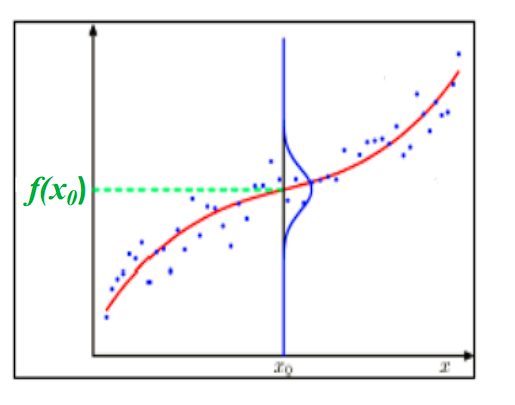
\includegraphics[width=0.5\textwidth]{assets/example/6.2.1.png}
\end{frame}

\begin{frame}{复杂表格}
    \begin{table}[htb]
        \centering
        \small
        \begin{tabular}{p{2.5cm}c{4cm}p{4cm}c{4cm}p{3.5cm}}
            \toprule
            \textbf{Layer} & \textbf{Channel in} & \textbf{Size in} & \textbf{Channel out} & \textbf{Size out}\\
            \midrule
            inc & 1 & $256\times256$ & 64 & $256\times256$\\
            \midrule
            down1 & 64 & $256\times256$ & 128 & $128\times128$\\
            down2 & 128 & $128\times128$ & 256 & $64\times64$\\
            down3 & 256 & $64\times64$ & 512 & $32\times32$\\
            down4 & 512 & $32\times32$ & 1024 & $16\times16$\\
            \midrule
            \multirow{2}{*}{up1} & 1024 & $16\times16$ & \multirow{2}{*}{512} & \multirow{2}{*}{$32\times32$}\\
             & 512 & $32\times32$ &  & \\
            \midrule
            \multirow{2}{*}{up2} & 512 & $32\times32$ & \multirow{2}{*}{256} & \multirow{2}{*}{$64\times64$}\\
             & 256 & $64\times64$ &  & \\
            \midrule
            \multirow{2}{*}{up3} & 256 & $64\times64$ & \multirow{2}{*}{128} & \multirow{2}{*}{$128\times128$}\\
             & 128 & $128\times128$ &  & \\
            \midrule
            \multirow{2}{*}{up4} & 128 & $128\times128$ & \multirow{2}{*}{64} & \multirow{2}{*}{$256\times256$}\\
             & 64 & $256\times256$ &  & \\
            \midrule
            out & 64 & $256\times256$ & 1 & $256\times256$\\
            \bottomrule
        \end{tabular}
    \end{table}
    \centering
    \small
    模型各层张量流向
\end{frame}

\begin{frame}{分栏}
    \begin{columns}
        \begin{column}{0.4\textwidth}
        \begin{center}
            \begin{minipage}{0.4\textwidth}
            \begin{enumerate}
                \item 有序列表1
                \item 有序列表2
                \begin{enumerate}
                    \item 有序子表
                    \item 有序子表
                \end{enumerate}
                \item ...
            \end{enumerate}
            \end{minipage}
        \end{center}
        \end{column}
        
        \begin{column}{0.6\textwidth}
            \centering
            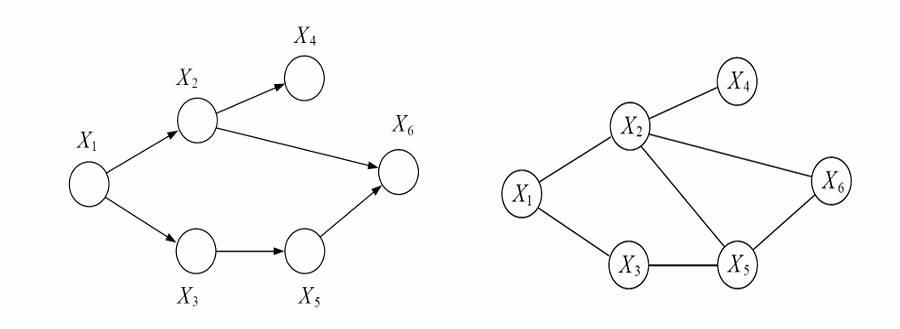
\includegraphics[width=\textwidth]{assets/example/11.1.1.png}\\
            图1
            \\
            
\includegraphics[width=\textwidth]{assets/example/11.2.1.png}\\
            图2
        \end{column}
    \end{columns}
\end{frame}

\section{进阶}
\begin{frame}{tikz例子}
    \begin{tikzpicture}[remember picture,overlay]
    
    \fill[yellow]
    (current page.west) rectangle (current page.south east);

    \node[anchor=center]
    at ([yshift=70pt, xshift=-300pt]current page.east) (side_pic_1) {
        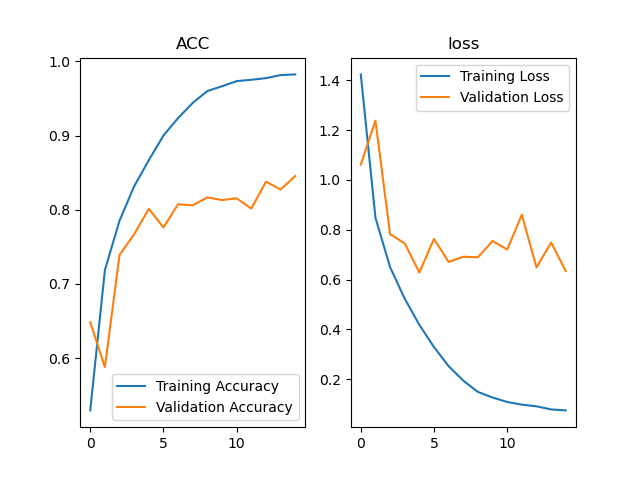
\includegraphics[width=0.3\textwidth]{assets/example/myplot.png}
    };

    \node[anchor=center]
    at ([yshift=70pt, xshift=300pt]current page.south west) (text_1) {
        \textcolor{black}{这是一段文本}
    };

    % -----两个node之间的箭头------
    \draw[->,line width =2pt,color=red] (text_1)--(side_pic_1);
    
    \end{tikzpicture}
\end{frame}
% ------------------------

\backmatter

\end{document}
